\section{弾性による高速化への影響}
\label{sec:elasticity-discussion}

\subsection{応力比と高速化度合の関係}
\ref{sec:viscosity}章にて示した通り,超音波照射された擬塑性流体中を落下する球の高速化の要因として粘性による影響では説明が十分にできない.球の落下速度が遅い場合,粘性以外の要因によって,超音波照射による落下球の高速化が抑制されていると考えられる.そこで,本章において先行研究である岩室\cite{ref:8}にて示唆されていた弾性による影響に関して考える.

\ref{sec:elasticity}節にて,貯蔵弾性率$G'$,損失弾性率$G''$と応力$\tau$の関係性を示した.また,弾性と粘性の支配要素が変わる応力$\tau_\text{0}$も示した.この応力$\tau_\text{0}$と式(\ref{eq:tauU})に示される,擬塑性流体中を落下する球によって生じる応力$\tau_\text{U}$の比$\tau_\text{U}/\tau_\text{0}$を用いて,超音波照射による球の高速化度合いを整理する.この比が1より大きいと粘性影響が,1より小さいと弾性影響が大きいと考えられる.この整理を行うことで,弾性による超音波照射された落下球の高速化度合いへの影響を考える.

応力比と終端速度の関係をFig\ref{fig:elastcity}(a)に示す.終端速度が速くなると,応力比が増加した.これは式(\ref{eq:tauU})において,擬塑性流体であるため$0<n<1$となり,終端速度が早くなると$\tau_\text{U}$が大きくなるためである.よって終端速度が速くなると粘性影響が大きく寄与することが分かる.

式(\ref{eq:muU}),(\ref{eq:muABL}),(\ref{eq:Udiff})より,終端速度$U_\text{off}$と高速化度合いの関係は,
\begin{eqnarray}
    \frac{U_\text{on}}{U_\text{off}} \sim U_\text{off}^{n-1} \left(\frac{1}{u}\right)^{n-1} \left(\frac{\delta}{a}\right)^n ,
    \label{eq:UTdiff_UT}
\end{eqnarray}
と見積もられる.擬塑性流体では$0<n<1$となるため,終端速度$U_\text{T}$の乗数は負となり,終端速度が遅い場合,高速化がより顕著に現れると考えられる.終端速度と高速化度合の関係をFig\ref{fig:elastcity}(b)に示す.終端速度が遅くなると高速化度合が大きくなったが,分散は大きい.これは終端速度だけでなく,音響境界層厚さの影響を受けるためと考えられる.

応力比と高速化度合いの関係を示した結果をFig\ref{fig:elastcity}(c),(d)に示す.Fig\ref{fig:elastcity}(c)は全ての実験結果を,Fig\ref{fig:elastcity}(d)はPAA濃度0.2wt.\%,岩室\cite{ref:8}以外の実験結果を示す.先行研究である岩室\cite{ref:8}の実験結果を含めた場合,明瞭な相関が見られない.球の落下による応力は超音波照射していない状態における終端速度にて定義しており,先行研究である岩室\cite{ref:8}は,照射する超音波周波数,平均圧力振幅,球径をパラメータとしているため,超音波周波数や平均圧力振幅を考慮していない落下球による応力比による整理では不十分であると考えられる.一方,今回の実験結果では応力比1近傍にて高速化が顕著に現れた.式(\ref{eq:tauU}),(\ref{eq:UTdiff_UT})より,終端速度が遅くなると球の落下による応力が小さくなり,高速化度合が大きくなる.しかし,応力比が1より小さくなると,高速化が抑制されていた.これは応力比が1を超えると,粘性ではなく弾性による支配が強くなるためと考えられる.ゆえに,弾性が支配的とならない応力比1近傍において高速化が顕著に現れたと考えられる.

\begin{figure}[H]
    \centering
    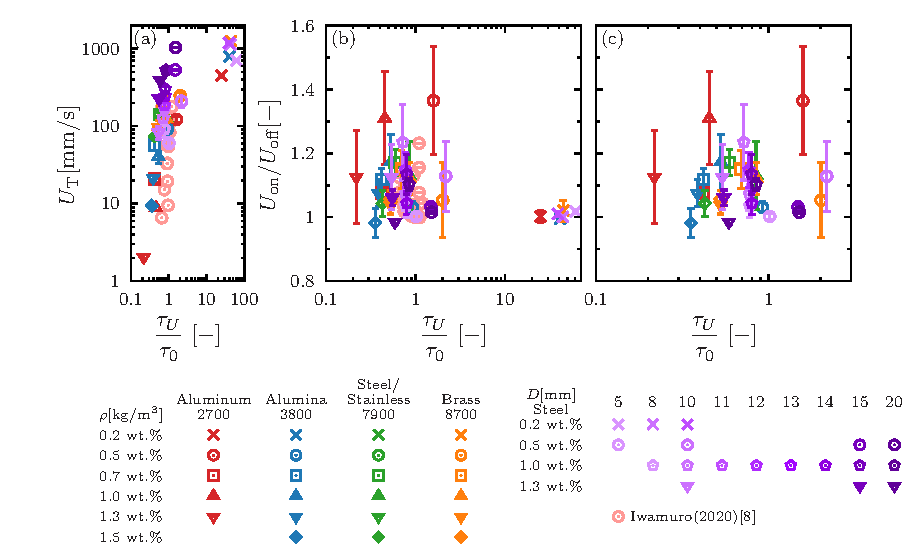
\includegraphics[width=1.0\textwidth]{5-Results/elastcity.eps}
    \caption{Relationship between terminal velocity and (a)elasticity ratio $\tau_\text{U}/\tau_\text{0}$, (b)velocity ratio, elasticity ratio $\tau_\text{U}/\tau_\text{0}$ and velocity ratio by (c)all experiment, (d)without 0.2wt.\% PAA solution.}
    \label{fig:elastcity}
\end{figure}

\subsection{粘度比・応力比による高速化への影響}
超音波照射による高速化に対する粘性と弾性の影響を考えるため,粘度比と音響境界層を球の半径で規格化した値と応力比,高速化度合の関係をFig\ref{fig:elastcityColor}に示す.縦軸は応力比,横軸は粘度比と音響境界層を球の半径で規格化した値,カラーバーは高速化度合を表す.粘度比と音響境界層を球の半径で規格化した値が増加すると,応力比が減少した.これは,粘度比が大きくなると,弾性による影響強くなることを示している.粘度比が大きくなるのは,式(\ref{eq:muU}),(\ref{eq:diff})より,終端速度が小さい場合である.終端速度が遅くなると,式(\ref{eq:tauU})より,球の落下による応力が小さくなり,粘度比と応力比の関係を示す.非常に粘度比が小さく,応力比が大きい領域では粘性による影響をあまり受けておらず,高速化が見られなかった.粘度比が増加して行くに従い応力比は減少し,粘度比0.1近傍,応力比1近傍にて高速化が顕著となった.その後,粘度比が0.1以上に増加した場合,応力比は1を下回り弾性による影響が支配的となったと考えられる.この領域において,高速化があまり見られなくなった.そして,粘度比1以上の領域では高速化が弱くみられるようになった.これは弾性が支配的ではあるものの,粘度比が大きいためと考えられる.以上より,粘度比と音響境界層を球の半径で規格化した値では高速化が単調増加せず,抑制される場合が存在したが,その要因は弾性による影響が強く現れたためと考えられる.

\begin{figure}[H]
    \centering
    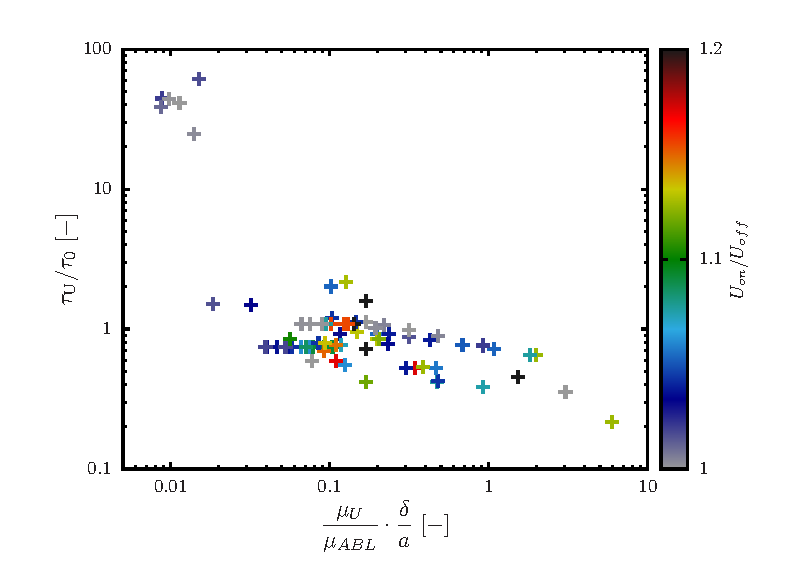
\includegraphics[width=0.9\textwidth]{5-Results/elastcity_color.eps}
    \caption{Relationship between velocity ratio and the inverse of the viscosity ratio multiplied by the thickness, elasticity ratio $\tau_\text{U}/\tau_\text{0}$.}
    \label{fig:elastcityColor}
\end{figure}
